\section{Evaluation}
\label{sec:evaluation}
We evaluate the reconstruction of physical identities and semantic events
from unperturbed recordings before examining its sensitivity to controlled
positioning and radar errors. We use the same recordings and
reconstruction settings in both parts.

\subsection{Experimental Setup}
\label{subsec:setup}
The dataset contains 19 scripted scenarios and 22 runs acquired in
CARLA~0.9.15 at 20~Hz~\cite{dosovitskiy2017carla,carla2023docs}.
The scenarios span three maps and cover rear-end, cut-in, junction and
chain collisions, occlusions, dense traffic and motorway driving. Across
the recordings, 50 recording and 45 non-recording vehicles are present,
with all 26 evaluated collisions occurring between recording vehicles.
Each recorder supplies
GNSS/INS poses, controls and indicators, impact reports without partner
identities, and three radar streams: a front radar with a 150$^\circ$
field of view and two side radars with 140$^\circ$, each with 90~m range
and 600 rays per sweep, and no rear coverage. G0 uses exact poses and native radar
returns without added corruption, although field of view, occlusion and
finite ray sampling still limit observations. By leaving impact-report
streams unchanged, the campaign tests collision matching under
positioning and radar errors rather than crash-sensor failures.

The position and heading perturbations in Table~\ref{tab:profiles}
combine constant bias, a Gauss--Markov component and white noise, while
velocity errors are white. G1 follows
measured RTK-INS accuracy~\cite{volckaert2019integrity}, and G2 uses
stronger targets informed by field trials and receiver
specifications~\cite{lesjak2025cits,ublox2024zedf9r}. The radar profiles
combine Gaussian measurement errors, independent return losses and
Poisson clutter, with values drawn from automotive measurements,
published models and engineering stress
choices~\cite{schumann2021radarscenes,scheel2019variational,kraus2021ghost}.
False-return locations are uniform over range and field of view, unlike
structured real clutter~\cite{kopp2021clutter}; the extreme clutter mean
serves as a model stress value, not an estimated deployment frequency.

\begin{table}[!t]
\caption{Added error profiles. Pose targets use the indicated percentiles.
Radar parameters are Gaussian standard deviations, per-return drop
probability $p$, and mean false returns per sweep per sensor $\lambda$;
$\sigma_{\angle}$ applies to both azimuth and elevation.}
\label{tab:profiles}
\centering
\footnotesize
\setlength{\tabcolsep}{3pt}
\begin{tabular*}{\columnwidth}{@{\extracolsep{\fill}}lccc@{}}
\hline
\textbf{Pose target} & \textbf{Position [m]} & \textbf{Heading [$^\circ$]} & \textbf{Velocity [m/s]} \\
\hline
G1 (P95) & 0.040 & 0.140 & 0.016 \\
G2 (P99.5) & 0.500 & 0.600 & 0.200 \\
\hline
\end{tabular*}
\smallskip
\begin{tabular*}{\columnwidth}{@{\extracolsep{\fill}}lccccc@{}}
\hline
\textbf{Radar} & $\sigma_\rho$ [m] & $\sigma_{\angle}$ [$^\circ$] & $\sigma_v$ [m/s] & $p$ & $\lambda$ \\
\hline
Nominal & 0.25 & 0.5 & 0.10 & 0.20 & 3 \\
Severe  & 0.50 & 2.0 & 0.20 & 0.40 & 3 \\
Extreme & 0.50 & 2.0 & 0.20 & 0.40 & 30 \\
\hline
\end{tabular*}
\end{table}

The experimental campaign comprises 1816 jobs covering G0,
positioning-only errors, radar errors and combined conditions.
All-recorder radar profiles affect every radar on every recording vehicle
throughout the log, while asymmetric jobs enumerate selected recorders
or subsets. Corresponding jobs use identical per-recorder perturbations,
but the pooled scenario weights differ: single-recorder rows contain one
job per recorder and all-recorder rows contain one per run. Stochastic
conditions use three seeds, or five for extreme radar. Reconstruction
results are averaged over seeds, and selected paired changes include
95\% Student's $t$ intervals over those seeds to quantify perturbation
variability on the designed cases.

Ground truth enters only at scoring, where physical association is
evaluated through correct, wrong and missed recorder links, entity
purity, false merges and fragmentation, independently of arbitrary
identifier names. Measured track samples are assigned to the nearest true
vehicle box within 1.5~m. Entity purity then measures the share carrying
the most frequent assignment, while an unmatched mode defines a phantom.
Position errors concern non-recording entities at states where the
contributing tracks agree with the same true vehicle, with impure states,
false entities and recorder duplicates counted separately.

To assess whether semantic conversion preserves the manoeuvres and
conflict timing needed to interpret the recorded sequence, local scoring
covers newly emitted path-entry, left/right cut-in and
\texttt{CRITICAL\_TTC} onsets. Predictions and oracle events are restricted
to before each recorder's first contact \emph{before} one-to-one matching
by type, physical subject and time within 2~s; witnesses without contact
contribute their full recording. Duplicate onsets count as false
positives, and precision and radar-observable recall pool these counts
across jobs. Since physical subjects are assigned from truth
correspondence, local event scores complement, rather than replace,
global association measures. The last-second diagnostic captures
unsupported context near impact by counting jobs with a nonduplicate
unmatched conflict interval overlapping $[t_c-1,t_c)$ before at least one
recorder's first contact.

\subsection{Reconstruction Across the Scenarios}
\label{subsec:exact}
Under G0, all 26 collision participant sets are correct and all 45
observable non-recording vehicles are represented, with median position
error 0.24~m (P95: 0.82~m) and median speed error 0.04~m/s. The physical
association results show correct recorder links in 49 cases, none wrong
and one missed. No false merge occurs, and measured-sample purity is 1.0
for 64 of 66 anonymous entities, with twenty duplicate entities and one
recorder duplicate counted separately. Together, these measures assess
consistency of physical identity independently of agreement between
local and global label names.

To assess the geometric reconstruction under G0, we compare the fitted
bodies with nominal boxes inferred independently from each source track.
The comparison pools 4376 source-consistent entity instants
across all 45 observable non-recording vehicles in the ten eligible runs.
At each instant, the reference is the median centre error over available
source boxes, and instants without a reference are excluded from both
sides. On this matched population, the combined body-reconstruction and
fusion step reduces median error from 0.484 to 0.240~m and P95 from
1.334 to 0.806~m. The median and P95 decrease in all ten runs, while
individual errors decrease at 81.4\% of paired instants.

Local conflict precision is 0.978 and observable recall 0.899
(Table~\ref{tab:results}), with a median matched onset error of 0.05~s.
The sequence recovered in S02 instantiates the running example: B enters
A's path just outside the following-distance reference, after which the
gap becomes unsafe and B's braking makes the predicted encounter
braking-critical. A's recorded brake command follows the first
reconstructed critical onset by 2.60~s, while cut-in, path-entry and
critical onsets agree with the oracle within 0.10~s. The chronology thus
recovers the gap left by B and the braking sequence that the final
contact alone does not preserve.

\begin{figure}[!t]
  \centering
  \setlength{\tabcolsep}{0pt}
  \begin{tabular}{c@{\hspace{4pt}}c}
    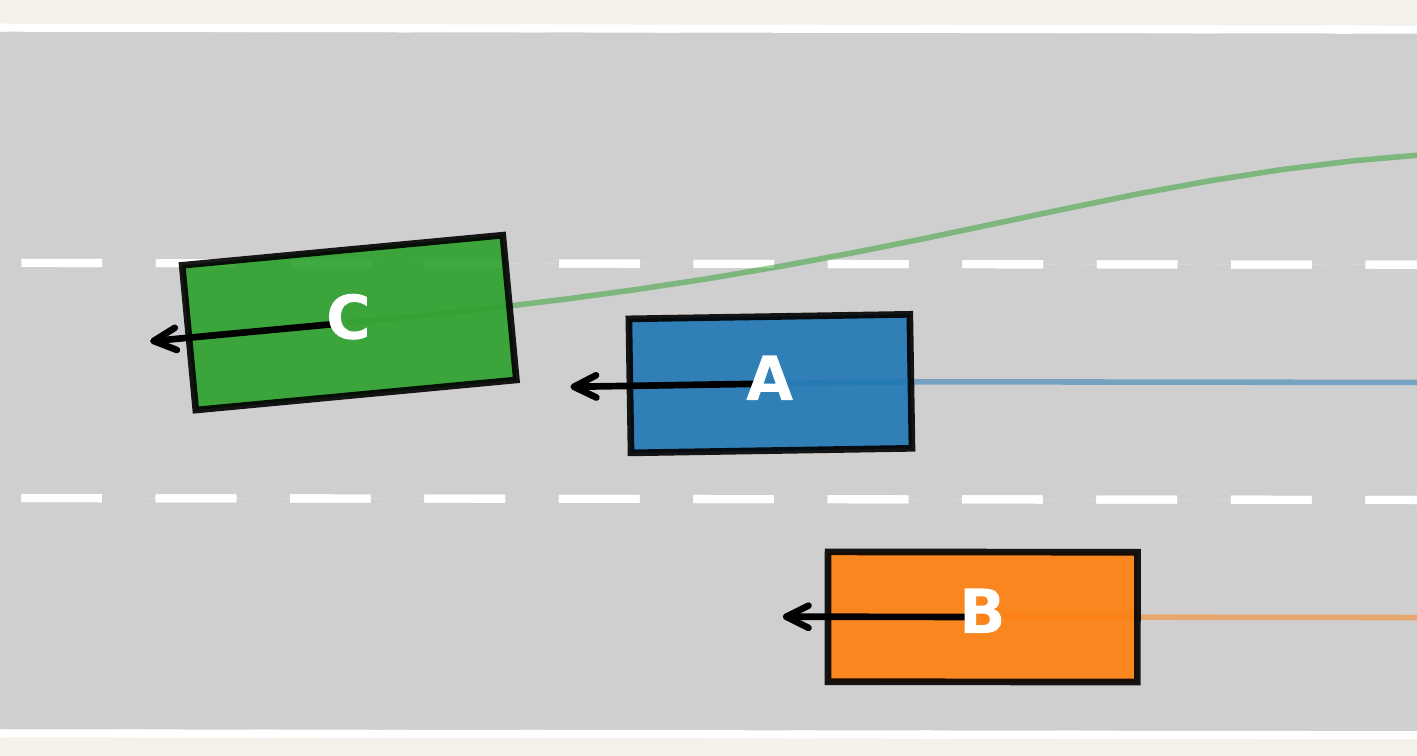
\includegraphics[width=0.485\columnwidth]{figures/viewer_s12_ground_truth.png} &
    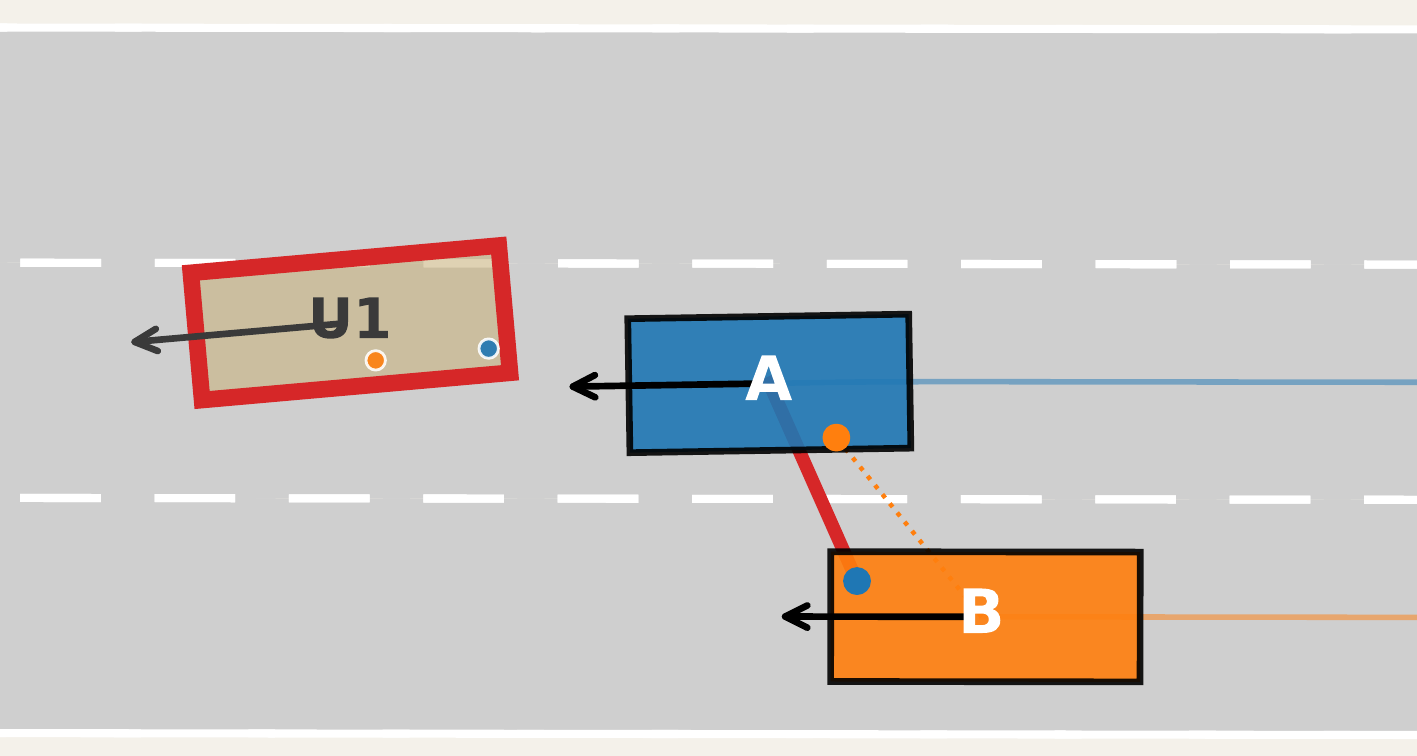
\includegraphics[width=0.485\columnwidth]{figures/viewer_s12_reconstruction.png} \\[1pt]
    {\scriptsize (a) Ground truth} & {\scriptsize (b) Reconstruction}
  \end{tabular}
  \caption{S12, one second before contact. C neither collides nor supplies a
  recording. Its radar observations from A and B form U1; red overlays
  show A's reconstructed conflicts with U1 and B.}
  \label{fig:viewer}
\end{figure}
Fig.~\ref{fig:viewer} shows how the reconstruction includes a vehicle
absent from the impact reports. In S12, C cuts into A's lane before A
swerves into B's lane and the two recorders collide. A's local evidence
already contains C's cut-in; association brings three tracks from A and
B into one road user, U1, with purity 1.0. By placing U1's cut-in and
path entry before A's critical interaction with B, the shared chronology
preserves both observers' evidence of the preceding interaction without
requiring a recording from C.

\subsection{Robustness to Sensor Degradation}
\label{subsec:robustness}

\begin{table*}[!t]
\caption{Selected conditions. Reconstruction columns are seed means;
local event scores are pooled counts. Coll.: fraction of correctly
identified contacts; Phant., Ghosts, W.~links and F.~merges: counts per job, with Ghosts
being recorders duplicated as anonymous entities; P95: source-consistent
road-user position error. Prec./Rec.: phase-restricted onset precision
and observable recall, including duplicate onsets as false positives.
Last 1~s: percentage of jobs with an unmatched nonduplicate interval overlapping the
second before a recorder's first contact.}
\label{tab:results}
\centering
\footnotesize
\setlength{\tabcolsep}{4pt}
\renewcommand{\arraystretch}{1.1}
\begin{tabular*}{\textwidth}{@{\extracolsep{\fill}}lrccccccccc@{}}
\hline
 & & \multicolumn{6}{c}{\textbf{Reconstruction}} & \multicolumn{3}{c}{\textbf{Local conflict events}} \\
\cline{3-8}\cline{9-11}
\textbf{Condition} & \textbf{Jobs} & \textbf{Coll.} & \textbf{Phant.} & \textbf{Ghosts} & \textbf{W.~links} & \textbf{F.~merges} & \textbf{P95 [m]} & \textbf{Prec.} & \textbf{Rec.} & \textbf{Last 1~s} \\
\hline
G0                &  22 & 1.000 &   0.0 & 0.05 & 0.00 & 0.00 & 0.82 & 0.978 & 0.899 &  4.5\% \\
G1, RTK           &  66 & 1.000 &   0.0 & 0.05 & 0.00 & 0.00 & 0.85 & 0.982 & 0.902 &  4.5\% \\
G2, degraded      &  66 & 1.000 &   0.0 & 0.02 & 0.00 & 0.00 & 0.87 & 0.986 & 0.906 &  3.0\% \\
Radar nominal     &  66 & 1.000 &   0.6 & 0.06 & 0.00 & 0.00 & 0.97 & 0.954 & 0.902 &  7.6\% \\
Radar severe      &  66 & 0.987 &  68.7 & 0.50 & 0.03 & 0.68 & 1.33 & 0.846 & 0.902 & 15.2\% \\
Radar extreme     & 110 & 0.954 & 102.4 & 1.79 & 0.12 & 0.91 & 1.56 & 0.313 & 0.834 & 86.4\% \\
One recorder, severe  & 150 & 0.995 & 30.5 & 0.26 & 0.01 & 0.03 & 1.08 & 0.911 & 0.892 &  8.7\% \\
One recorder, extreme & 250 & 0.981 & 45.6 & 0.84 & 0.05 & 0.06 & 1.19 & 0.509 & 0.862 & 56.8\% \\
G2 + radar severe &  66 & 1.000 &  69.6 & 0.52 & 0.03 & 0.73 & 1.33 & 0.826 & 0.879 & 25.8\% \\
\hline
\end{tabular*}
\end{table*}

Positioning errors under G1 and G2 preserve correct identification of
every collision and representation of every observable non-recording
vehicle, with neither wrong recorder links nor false merges. The paired
changes in road-user P95 are also small: G1 adds 0.031~m (95\% CI:
$[-0.027,0.089]$~m), and G2 adds 0.050~m ($[-0.075,0.175]$~m). Nominal
radar likewise preserves collision identification, with position P95
below 1~m. Position errors, false entities and association errors increase
under severe and extreme radar, although the all-recorder tests retain
98.7\% and 95.4\% correct collision participant sets, respectively.
Across the entire campaign, all 2344 true contact instances are detected
and 2322 have correct participant sets; 22 extra single-recorder impact
nodes are also produced. Reporting these outcomes separately keeps
collision identification distinct from radar identities and semantic
correctness.

In the asymmetric rows, severe corruption of one recorder retains
99.5\% correct collision sets, while extreme corruption reduces local
event precision to 0.509. Adding G2 to all-recorder severe
radar changes position P95 little but reduces local precision from 0.846
to 0.826. The sustained all-recorder profiles, which leave no unaffected
radar observer, characterize stress sensitivity rather than the
frequency of simultaneous failures.

Two supplementary tests perturb the clocks and the impact reports,
using three seeds per run under G0 and G2 with severe radar.
Clock offsets drawn uniformly within $\pm50$~ms per recorder
are recovered within $0.1$~ms for successfully aligned recorders;
one of $150$ recorders loses radar-based alignment under G2
with severe radar. Reconstructed event times nevertheless
shift by up to $0.3$~s under G0 and $0.75$~s under G2 with
severe radar, reversing $0.25\%$ and $0.40\%$ of the evaluated
event-pair orderings, respectively. EDR-inspired impact
reports are perturbed with $\Delta V$ noise having $5\%$ or
$10\%$ standard deviation per impact, compared with the
$\pm10\%$ measurement accuracy specified in US
regulations~\cite{cfr563}, together with $5\%$ mass error
per recorder and up to $\pm10$~ms of timing error.
Collision participant sets remain correct in all
$264$ impact-perturbation jobs.

\subsection{Reliability of the Event Chronology}
\label{subsec:chronology}
For the surrounding chronology, positioning-only and nominal-radar
conditions retain local conflict precision above 0.95 and observable
recall near 0.90, accompanied by a median matched onset error of 0.05~s
and median matched interval overlap of about 0.97. With one severely
degraded recorder, precision is 0.911 and 8.7\% of jobs contain an
unmatched nonduplicate interval in the last second before a recorder's
first contact; with all recorders severely degraded, these values become
0.846 and 15.2\%.

The distinction between collision identification and contextual evidence
becomes more pronounced under extreme radar. With every recorder
affected, precision falls to 0.313 while observable recall remains 0.834,
and 793 of 907 false predictions concern phantom subjects. Median matched
onset error remains 0.10~s, but this timing accuracy applies to matched
events and does not validate the unmatched ones. Last-second unmatched
intervals occur in 86.4\% of jobs, and even one extremely degraded
recorder gives 56.8\%. The chronology therefore preserves many genuine
conflicts while adding substantial unsupported context under dense
clutter. Its claims remain auditable through recorder provenance,
original local events and retrospective identity evidence, with their
reliability assessed through the separate association and event-quality
measurements.
